\chapter{几何Satake等价I：球面Hecke代数的范畴化}\label{L21}\lecturedate{2020/04/29}\sourcepage{173}
Satake同构有一个优美的几何版本。本课程最后三讲将围绕这一主题展开，主要遵循Mirković与Vilonen的论文\bref{L21MV}{MV}。

首先回顾，为表述$\GL_n$的几何Langlands对应，我们已经做了哪些工作。
\begin{enumerate}[label=\arabic*.]
\item 选取复数域或有限域上曲线$X$的函数域作为基础域$F$。
\item 找到合适的几何空间$\operatorname{Bun}_X$；其向量丛同构类集合可识别为$\GL_n(F)\backslash\GL_n(\A_F)/K$。
\item 借助Grothendieck的“函数—层”字典，把$\GL_n(F)\backslash\GL_n(\A_F)/K$上的Hecke特征函数替换为$\operatorname{Bun}_X$上的Hecke特征层，也就是相应的反常层。
% [Tutor Note: 原书 p173 作 “perverse sheaves over G”，其中 $G$ 系 $\operatorname{Bun}_X$ 之误（该条讲的是 $\operatorname{Bun}_X$ 上的 Hecke 特征层）；译文按 $\operatorname{Bun}_X$ 处理。]
\item 把Galois表示替换为平展基本群$\widehat\pi_1(X)$的表示。
\item 几何表述为：$\widehat\pi_1(X)$的不可约秩$n$表示对应于$\operatorname{Bun}_X$上的Hecke特征层，如下图所示。
\end{enumerate}
\begin{figure}[H]\centering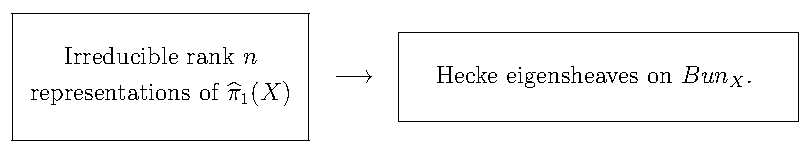
\includegraphics[width=0.6543\paperwidth]{images/L21-p173-correspondence.pdf}\end{figure}
\sourcepage{174}
不过，Satake同构是一个局部命题，因此不需要类似曲线$X$这样的整体对象；即使存在曲线$X$，我们也只考察某一点$x\in X$附近的局部结构。对偶群$G^L$与$G$的\textbf{仿射Grassmannian}\znote{仿射 Grassmannian 是 $\operatorname{Bun}_X$ 的局部模型：在曲线一点附近，向量丛的变形只由 $G(\mathcal K)$ 模 $G(\mathcal O)$ 的等价类刻画。普通 Grassmannian 参数化向量空间的子空间；把向量空间换成形式 Laurent 级数域上的格，就得到仿射版本，名字由此而来。它与对偶群 $G^L$ 一起，在 Satake 对应中分别扮演 $\operatorname{Bun}_X$ 与 $\widehat\pi_1(X)$ 的角色。[来源：nLab "affine Grassmannian"，\url{https://ncatlab.org/nlab/show/affine+Grassmannian}（Last revised 2023-08-15；2026-11-14 访问）。]}将分别扮演类似于$\widehat\pi_1(X)$和$\operatorname{Bun}_X$的角色。

设$G$为有限域$\F_q$或复数域$\C$上的连通分裂约化群。令$\mathcal O=\F_q[[t]]$或$\C[[t]]$，相应地$\mathcal K=\F_q((t))$或$\C((t))$。正环群$G(\mathcal O)$及商$G(\mathcal K)/G(\mathcal O)$具有群概形和ind概形结构；后者记为$\operatorname{Gr}$，即仿射Grassmannian。设$k$为具有有限整体维数的Noether交换含幺环，例如$\C,\Z,\F_q$。以$P_{G(\mathcal O)}(\operatorname{Gr},k)$表示$k$系数的$G(\mathcal O)$等变反常层范畴，以$\operatorname{Rep}G^L_k$表示对偶分裂约化$k$群概形的有限生成$k$表示范畴。几何Satake等价\znote{它把第 19 讲的 Satake 同构在范畴层面提升：不再比较两边的环，而是比较两个张量范畴。易错点：使左边成为对称张量范畴所需的交换约束并非卷积结构自动给出，而是额外的数据，这是本等价最微妙之处。[来源：nLab "geometric Satake equivalence"，\url{https://ncatlab.org/nlab/show/geometric+Satake+equivalence}（Last revised 2024-07-22；2026-11-14 访问）。]}为下列定理。
\originalnumber{1}
\begin{theorem}\label{L21S0O1}
范畴$P_{G(\mathcal O)}(\operatorname{Gr},k)$与$\operatorname{Rep}G^L_k$作为张量范畴等价。
\end{theorem}\idx{几何Satake等价}\idx{仿射Grassmannian}
\section{仿射Grassmannian}\label{L21S1}
为了遵循Mirković–Vilonen的论述并使叙述简明，以下几何基础域始终取$\C$。不过，整个理论的大部分可在整数上建立，见\bref{L21MV}{MV}第14节。若希望了解这里列出的仿射Grassmannian性质的详细证明，可参看\bref{L21BD}{BD}第4.5节。

设$G$为$\C$上的连通约化群。以$\mathcal R$表示Noether交换含幺$\C$代数的范畴。$G$的仿射Grassmannian$\operatorname{Gr}=\operatorname{Gr}_G$是$\C$上的 ind 有限型 ind 概形\znote{ind 概形是概形范畴中的 ind-对象，即按闭嵌入取滤过的正向极限 $\varinjlim_nX_n$。它比有限型概形大得多，正因如此才能在第 3 节用直接极限定义整体的反常层范畴；形式环空间常是 ind 概形而并非概形。对仿射 Grassmannian，$X_n$ 可取第 1 节式 (1.1) 中的有限型闭子概形 $\operatorname{Gr}^n$。[来源：nLab "ind-scheme"，\url{https://ncatlab.org/nlab/show/ind-scheme}（Last revised 2023-11-11；2026-11-14 访问）。]}，代表以下函子$\operatorname{Gr}_G:\mathcal R\to\mathbf{Sets}$：
\[\operatorname{Gr}_G(R)=\left\{(\mathcal P,\alpha)\ \middle|\ \begin{array}{l}\mathcal P\text{ 是 }\Spec R[[t]]\text{ 上的主 }G\text{ 丛},\\\alpha:\mathcal P|_{\Spec R((t))}\xrightarrow{\sim}\mathcal P^0|_{\Spec R((t))}\end{array}\right\}\big/\text{同构},\]
其中$\mathcal P^0=G\times\Spec R[[t]]$为$\Spec R[[t]]$上的平凡$G$丛。
\sourcepage{175}
令$\mathcal K=\C((t))$，$\mathcal O=\C[[t]]$。以下引理解释了为什么$\operatorname{Gr}$是几何框架中$\operatorname{Bun}_X$的局部对应物。
\originalnumber{1}
\begin{lemma}\label{L21S1O1}$G(\mathcal K)/G(\mathcal O)$与$\operatorname{Gr}_G(\C)$之间存在自然双射。\end{lemma}
\begin{proof}
当剩余域为代数闭域时，$\Spec k[[t]]$上的每个$G$丛都可平凡化。因此，$\Spec\mathcal O$上的$G$丛$\mathcal P$可选取平凡化$\beta:\mathcal P\xrightarrow{\sim}\mathcal P^0$。每个$(\mathcal P,\alpha)\in\operatorname{Gr}_G(\C)$便给出$\mathcal P^0|_{\Spec\mathcal K}$的自同构$\alpha\circ\beta^{-1}|_{\Spec\mathcal K}\in G(\mathcal K)$。改变$\beta$仅改变其右侧的$G(\mathcal O)$因子，因而得到唯一确定的右陪集。这就证明了引理。
% [Tutor Note: 原书 p175 证明中作 $\beta^{-1}|_{\Spec\mathcal K}\circ\alpha^{-1}$，但 $\beta^{-1}\circ\alpha^{-1}$ 的余域是 $\mathcal P$ 而非 $\mathcal P^0$，不能视为 $G(\mathcal K)$ 的元素；译文按 $\alpha\circ\beta^{-1}|_{\Spec\mathcal K}$ 处理。]
\end{proof}
\originalnumber{2}
\begin{note}[L21S1O2]
\begin{enumerate}[label=(\arabic*)]
\item 若$G$在$\Z$上定义，则$\operatorname{Gr}_G$也可在$\Z$上定义。
\item 若$F$为非阿基米德局部域，$\OO_F$为其整数环，剩余域为$\F_q$，并给$G$选定合适的光滑连通$\OO_F$模型，则相应局部仿射Grassmannian也满足$G(F)/G(\OO_F)\cong\operatorname{Gr}_G(\F_q)$。
\end{enumerate}
\end{note}
函子$\operatorname{Gr}_G$由ind有限型且ind射影的ind概形代表，是一个不平凡的事实。下面说明其约化结构：$\operatorname{Gr}(\C)$可以写成一族在$\C$上射影、有限型的闭约化子概形的并。

由于可取嵌入$G\hookrightarrow\GL_n$，只需对$\GL_n$说明这一构造。此时$\GL_n(\mathcal O)\cong\operatorname{Aut}(\mathcal O^{\oplus n})$。对正整数$s$，定义有界格的集合
\begin{equation}\tag{1.1}\label{L21eq11}\operatorname{Gr}^{s}:=\{g\mathcal O^{\oplus n}\mid g\in\GL_n(\mathcal K),\ t^s\mathcal O^{\oplus n}\subseteq g\mathcal O^{\oplus n}\subseteq t^{-s}\mathcal O^{\oplus n}\}.\end{equation}
显然$\operatorname{Gr}(\C)=\bigcup_{s\ge0}\operatorname{Gr}^s$。另一方面，$V:=t^{-s}\mathcal O^{\oplus n}/t^s\mathcal O^{\oplus n}\cong\C^{2sn}$，因而有映射
\[\operatorname{Gr}^s\to\operatorname{Gr}(\cdot,V):=\bigsqcup_{0\le m\le2sn}\operatorname{Gr}(m,V),\qquad g\mathcal O^{\oplus n}\longmapsto g\mathcal O^{\oplus n}/t^s\mathcal O^{\oplus n},\]
这里$\operatorname{Gr}(m,V)$为向量空间$V$的通常Grassmannian。该映射把有界格空间的约化结构实现为$\operatorname{Gr}(\cdot,V)$的闭约化子概形，因此它射影且有限型。其像作为点集恰为
\[\operatorname{Gr}(\cdot,V)^t=\{W\subseteq V\mid tW\subseteq W\}.\]

\originalnumber{3}
\begin{note}[L21S1O3]仿射Grassmannian 的 ind 概形本身约化，当且仅当$\operatorname{Hom}(G,\mathbb G_m)=0$，见\bref{L21BD}{BD}的定理4.5.1。\end{note}
Beauville–Laszlo还给出了$\operatorname{Gr}_G$的另一种解释。设$C$为域$k$上的曲线，例如$k=\C$或$\F_q$。固定一个光滑$k$有理点$x\in C$，并选取$x$处的局部参数。
\sourcepage{176}
令$C^*=C\setminus\{x\}$。定义函子$\operatorname{Gr}_{G,x}:\mathcal R\to\mathbf{Sets}$：
\[\operatorname{Gr}_{G,x}(R)=\left\{(\mathcal P,\alpha)\ \middle|\ \begin{array}{l}\mathcal P\text{ 是 }C_R\text{ 上的 }G\text{ 丛},\\\alpha:\mathcal P|_{C^*_R}\xrightarrow{\sim}G\times C^*_R\end{array}\right\}\big/\text{同构}.\]
\originalnumber{4}
\begin{theorem}[Beauville–Laszlo]\label{L21S1O4}$\operatorname{Gr}_{G,x}$与$\operatorname{Gr}_G$同构。\end{theorem}
\section{仿射Grassmannian的胞腔}\label{L21S2}\idx{环群}\idx{半无限轨道}
以下讨论约化ind概形及其经典拓扑。设$Z(G)$为$G$的中心，$Z=Z(G)^0$为中心中包含单位元的连通分支，令$\bar G=G/Z$。则有非典范同构
\begin{equation}\tag{2.1}\label{L21eq21}(\operatorname{Gr}_G)_{\mathrm{red}}\cong\operatorname{Gr}_{\bar G}\times X^\vee(Z),\end{equation}
其中$X^\vee(Z)=\operatorname{Hom}(\C^\times,Z)$。
% [Tutor Note: 原书 p176 的 (2.1) 未标约化，直接写作 $\operatorname{Gr}_G\cong\operatorname{Gr}_{\bar G}\times X^\vee(Z)$；当 $Z\ne1$ 时 $\operatorname{Gr}_G$ 可以非约化，译文按约化结构 $(\operatorname{Gr}_G)_{\mathrm{red}}$ 处理。]

$G(\mathcal K)$也称为$G$的\textbf{环群}\znote{「环群」有拓扑与代数两层含义：拓扑上是自由环空间 $\mathcal LG=\operatorname{Map}(S^1,G)$，可分解为 $G\times\Omega G$（基于环空间），其表示论远比 $G$ 丰富；代数上则指形式 Laurent 级数的点 $G(\mathcal K)$。本讲的中心扩张与 Kac--Moody 代数都属于代数版本。注意代数版本只取形式 Laurent 级数的点，不是拓扑极限。[来源：nLab "loop group"，\url{https://ncatlab.org/nlab/show/loop+group}（Last revised 2026-03-21；2026-11-14 访问）。]}。设$\Gamma\cong\C^\times$为$\operatorname{Aut}(\mathcal K)$中按$t\mapsto st$作用的子群，其中$s\in\Gamma$。$\Gamma$也作用于$G(\mathcal O)$和$G(\mathcal K)$，因而可组成半直积
\[\widetilde G(\mathcal K):=G(\mathcal K)\rtimes\Gamma,\]
其中包含Cartan子群$T\times\Gamma$，$T$为$G$的极大环面。相应的\textbf{仿射Kac–Moody群}$\widehat G(\mathcal K)$为$\widetilde G(\mathcal K)$的一个中心扩张\znote{中心扩张是短正合列 $1\to A\to\widehat G\to G\to1$，且 $A$ 的像落在 $\widehat G$ 的中心。对环群 $G(\mathcal K)$，其中心扩张的 Lie 代数正是下面的 $\widehat{\g}$：扩张的核 $\mathbb G_m$ 对应中心元 $c$，其系数通常称为能级。扩张的存在性依赖 $G$ 上的不变双线性型（Killing 型即可）；换用另一个双线性型相当于把 $c$ 乘上常数，故扩张按该常数分类，这个常数就是能级。[来源：nLab "group extension"，\url{https://ncatlab.org/nlab/show/group+extension}（Last revised 2026-02-23；2026-11-14 访问）。]}：
\[1\to\mathbb G_m\to\widehat G(\mathcal K)\to\widetilde G(\mathcal K)\to1.\]
其Lie代数为Kac--Moody 代数\znote{$\widehat{\g}$ 是最重要的一类 Kac--Moody 代数，即仿射型：它由环代数 $\g((t))$ 添上中心元 $c$ 与导出元 $d$ 得到，可看成环群的切代数加上与量子化（量子异常）有关的修正项；添 $d$ 是为了让 $\delta$ 成为 $\widehat{\mathfrak h}$ 上真正的根，从而得到与有限维情形平行的根空间分解。[来源：nLab "affine Lie algebra"，\url{https://ncatlab.org/nlab/show/affine+Lie+algebra}（Last revised 2024-12-08；2026-11-14 访问）。]}
\[\widehat{\g}=\g((t))\oplus\C c\oplus\C d,\]
Lie括号由下式给出：
\begin{align*}
[x(t),y(t)]&=[x(t),y(t)]_{\g}+\operatorname{Res}_{t=0}\left(\frac{dx(t)}{dt},y(t)\right)dt\,c,\\
[d,x(t)]&=t\frac{dx(t)}{dt},\\
[x(t),c]&=0=[d,c].
\end{align*}
这里$[-,-]_{\g}$为$\g$上的Lie括号在$\g((t))$上的延拓，$(-,-)$为$\g$上的不变双线性型；例如Killing型。
\sourcepage{177}
Cartan子代数为$\widehat{\mathfrak h}=\mathfrak h\oplus\C c\oplus\C d$，其中$\mathfrak h$为$\g$的Cartan子代数。根集合为
\[\widehat\Phi=\{\alpha+m\delta\mid\alpha\in\Phi\cup\{0\},\ m\in\Z\}\setminus\{0\},\]
其中$\delta$为$\widetilde T=T\times\Gamma$的特征标，在$T$上平凡，在$\Gamma$上为恒等特征标。选取$B\supseteq T$，并记其幂幺根基为$N$。$B$中的根就是$G$的正根。$\widehat G(\mathcal K)$的正根集合定义为
\[\widehat\Phi_+=\{\alpha+m\delta\mid\alpha\in\Phi_+,\ m\ge0\}\cup\{\alpha+n\delta\mid\alpha\in\Phi_-\cup\{0\},\ n>0\}.\]
% [Tutor Note: 原书 p177 正根定义中两个集合的哑标都写作 $k$（$k\ge0$ 与 $k>0$），译文分别改用 $m,n$ 以免混淆。]
以$\delta^\vee$表示$\Gamma\hookrightarrow\widetilde T$这一余特征标。

群概形$G(\mathcal O)$以左乘方式作用于$\operatorname{Gr}$，其轨道均为有限维。设$\lambda\in X^\vee(T)$为$T$的余特征标。它在$\mathcal K$值点上给出同态$\lambda_t:\mathcal K^\times\to T(\mathcal K)$。其伴随作用满足
\[\operatorname{Ad}_{\lambda_t(at^m)}(x_\alpha\otimes t^n)=a^{\langle\alpha,\lambda\rangle}x_\alpha\otimes t^{n+m\langle\alpha,\lambda\rangle},\qquad a\in\C^\times,\ m,n\in\Z,\ x_\alpha\in\g_\alpha.\]
% [Tutor Note: 原书 p177 的伴随作用公式右端作 $t^{n+\langle\alpha,\lambda\rangle}$，漏掉了 $at^m$ 中 $t^m$ 贡献的因子；译文按 $t^{n+m\langle\alpha,\lambda\rangle}$ 处理。]
记$t^\lambda=\lambda_t(t)$，并以$L_\lambda=t^\lambda G(\mathcal O)\in\operatorname{Gr}(\C)$表示对应的点。令$\operatorname{Gr}_\lambda$为包含$L_\lambda$的$G(\mathcal O)$轨道。于是$\operatorname{Gr}=\bigcup_{\lambda\in X^\vee}\operatorname{Gr}_\lambda$。设$W$为$T$的Weyl群。由Bruhat分解，$L_{w(\lambda)}$与$L_\lambda$位于同一$G(\mathcal O)$轨道，因此这些轨道由$X^\vee(T)$中的$W$轨道参数化，即
\[\operatorname{Gr}=\bigsqcup_{\lambda\in(X^\vee)^+}\operatorname{Gr}_\lambda.\]
这也称为Cartan分解\znoteplain{这里有两种「分解」，不要混淆：$\operatorname{Gr}=\bigsqcup_\lambda\operatorname{Gr}_\lambda$ 是按 $G(\mathcal O)$ 轨道（按支配余权）的分解，原书 p177 称之为 Cartan 分解（文献中亦用此名，此处按原书用词）；第 2 节末所说的胞腔分解，则是 $G/P_\lambda$ 的 Bruhat 胞腔（$G=\bigsqcup_{w}BwB$）沿纤维丛拉回所得。前者不是胞腔分解：每个 $G(\mathcal O)$ 轨道本身仍是有限维簇；正是这一有限维性使第 2 节能用有限维子簇的极限来刻画 $\operatorname{Gr}$。（上下文推断，无外部依据）}。由环旋转$t\mapsto st$诱导的$\C^\times$作用，其不动点集恰为$\bigsqcup_{\lambda\in(X^\vee)^+}G\cdot L_\lambda$。根据Białynicki–Birula定理，见\bref{L21B}{B}的定理4.1，可进一步得到下列命题。
\originalnumber{1}
\begin{proposition}\label{L21S2O1}
对支配余权$\lambda$，在$t=0$处求值的映射$\operatorname{ev}:G(\mathcal O)\to G$诱导的自然投影$\operatorname{Gr}_\lambda\to G\cdot L_\lambda$为纤维丛，其纤维同构于$\ker(\operatorname{ev})\cdot L_\lambda$。特别地，$\dim\operatorname{Gr}_\lambda=2\langle\kappa,\lambda\rangle$，其中$\kappa$为所有正根之和的一半。
\end{proposition}
注意，$\ker(\operatorname{ev})$为正同余群，其Lie代数为$t\g[[t]]$。选取有序根群坐标后，轨道纤维的坐标由
\[\bigoplus_{\substack{\alpha\in\Phi\\0<m<\langle\alpha,\lambda\rangle}}\g_\alpha\otimes t^m\]
给出，因此
\[\ker(\operatorname{ev})\cdot L_\lambda\cong\C^{\sum_{\alpha\in\Phi,\ \langle\alpha,\lambda\rangle>0}(\langle\alpha,\lambda\rangle-1)}.\]
\sourcepage{178}
令$n_\lambda=\sum_{\alpha\in\Phi,\ \langle\alpha,\lambda\rangle>0}(\langle\alpha,\lambda\rangle-1)$，则$\operatorname{Gr}_\lambda\to G\cdot L_\lambda$为$\C^{n_\lambda}$纤维丛。又$G\cdot L_\lambda\cong G/P_\lambda$，其中$P_\lambda$为$L_\lambda$的稳定子群，是由
\[\Delta_\lambda=\{\alpha\text{ 为单根}\mid\langle\alpha,\lambda\rangle=0\}\]
确定的、与相应标准抛物子群相反的抛物子群；标准抛物子群的定义见\sref{L19S1}。
% [Tutor Note: 原书 p178 称 $P_\lambda$ 为 $\Delta_\lambda$ 确定的 “standard parabolic subgroup”；但按正文 $G(\mathcal O)$ 左乘 $G(\mathcal K)/G(\mathcal O)$ 的约定，$L_\lambda$ 的稳定子是与标准抛物子群相反的抛物子群（例如 $G=\operatorname{SL}_2$、$\lambda$ 正则支配时稳定子为 $B^-$），译文按此处理。]因此
\[\dim G\cdot L_\lambda=|\{\alpha\in\Phi\mid\langle\alpha,\lambda\rangle<0\}|,\]
且
\[\dim\operatorname{Gr}_\lambda=\sum_{\substack{\alpha\in\Phi\\\langle\alpha,\lambda\rangle>0}}\langle\alpha,\lambda\rangle=2\langle\kappa,\lambda\rangle,\]
因为配对为负与为正的根的个数相同。Bruhat分解给出$G/P_\lambda$的胞腔分解，从而也给出每个$G(\mathcal O)\cdot L_\lambda$的胞腔分解。
\originalnumber{2}
\begin{proposition}\label{L21S2O2}
对支配余权$\gamma,\lambda$，$\operatorname{Gr}_\gamma\subseteq\overline{\operatorname{Gr}_\lambda}$当且仅当$\gamma\le\lambda$，即$\lambda-\gamma$为正余根的非负整系数和。
\end{proposition}
\originalnumber{3}
\begin{note}[L21S2O3]
\begin{enumerate}[label=(\arabic*)]
\item 严格来说，Białynicki–Birula定理用于代数簇，而不能直接用于整个ind概形。不过，可以在所需的有限维轨道及适当的有限维部分上应用这一方法。
\item 还存在反向Cartan分解：$\operatorname{Gr}=\bigsqcup_{\lambda\in(X^\vee)^+}\operatorname{Gr}^-_\lambda$，其中$\operatorname{Gr}^-_\lambda=G(\C[t^{-1}])\cdot L_\lambda$。在$t^{-1}=0$处求值诱导投影$\operatorname{Gr}^-_\lambda\to G\cdot L_\lambda$。在非平凡半单情形，纤维为无限维；其在$L_\lambda$处的切空间方向由
\[\mathfrak h\otimes t^{-1}\C[t^{-1}]\ \oplus\!\bigoplus_{\substack{\alpha\in\Phi\\m<\min\{0,\langle\alpha,\lambda\rangle\}}}\g_\alpha\otimes t^m\]
描述。
% [Tutor Note: 原书 p178 的 Remark 2.3(2) 只写出根空间部分 $\bigoplus_{\alpha\in\Phi,\ m<\min\{0,\langle\alpha,\lambda\rangle\}}\g_\alpha\otimes t^m$，略去了环面方向 $\mathfrak h\otimes t^{-1}\C[t^{-1}]$；译文补全了切空间的方向分解。]
\end{enumerate}
\end{note}
对于秩$r$的环面，$T(\mathcal O)\cong(\C[[t]]^\times)^r\cong(\C^\times)^r\times(1+t\C[[t]])^r$。每个余特征标都诱导$\operatorname{Gr}$上的$\C^\times$作用。考虑$2\kappa^\vee$所诱导的作用，不动点集为$\{L_\lambda\mid\lambda\in X^\vee\}$。% [Tutor Note: 原书 p178 作 $T(\mathcal O)\cong(\C[[t]]^\times)^r=(\C^\times)^r$，但 $\C[[t]]^\times\ne\C^\times$（还差主单位部分 $1+t\C[[t]]$）；译文按 $(\C^\times)^r\times(1+t\C[[t]])^r$ 处理。]
相应的吸引集与排斥集为
\[\operatorname{Gr}^{2\kappa^\vee,+}_\gamma=S_\gamma:=N(\mathcal K)\cdot L_\gamma,\qquad\operatorname{Gr}^{2\kappa^\vee,-}_\gamma=T_\gamma:=N^-(\mathcal K)\cdot L_\gamma,\]
其中$N^-$为$N$在Cartan对合下的像。最终得到Iwasawa分解
\[\operatorname{Gr}=\bigsqcup_{\gamma\in X^\vee}S_\gamma,\qquad\operatorname{Gr}=\bigsqcup_{\gamma\in X^\vee}T_\gamma.\]
这些半无限轨道$S_\gamma,T_\gamma$一般既不是有限维，也不是有限余维；但它们与$\overline{\operatorname{Gr}_\lambda}$的交是代数簇。
\originalnumber{4}
\begin{proposition}\label{L21S2O4}
\begin{enumerate}[label=(\arabic*)]
\item $\overline{S_\gamma}=\bigcup_{\nu\le\gamma}S_\nu$。
\item 把$\operatorname{Gr}$嵌入适当的ind射影空间后，$\overline{S_\gamma}$中$S_\gamma$的边界由一个超平面截面给出。
\end{enumerate}
\end{proposition}
为了构造第二条所需的嵌入，先归约到$G$单且单连通的情形，此时$\operatorname{Pic}(\operatorname{Gr})\cong\Z$。
\sourcepage{179}
设$\mathcal L$为$\operatorname{Pic}(\operatorname{Gr})$的丰沛生成元。仿射Kac–Moody群$\widehat G(\mathcal K)$作用于$H^0(\operatorname{Gr},\mathcal L)^\vee$，由此诱导$G(\mathcal K)$等变嵌入
\[\operatorname{Gr}\hookrightarrow\mathbb P\bigl(H^0(\operatorname{Gr},\mathcal L)^\vee\bigr).\]
% [Tutor Note: 原书 p179 写作 $\operatorname{Gr}\hookrightarrow\mathbb P(H^0(\operatorname{Gr},\mathcal L))$；由整体截面的求值映射得到的嵌入应取对偶空间 $\mathbb P(H^0(\operatorname{Gr},\mathcal L)^\vee)$，译文按后者处理。]
\originalnumber{5}
\begin{theorem}\label{L21S2O5}
设$\lambda$为支配余权。
\begin{enumerate}[label=(\arabic*)]
\item $S_\gamma\cap\overline{\operatorname{Gr}_\lambda}$非空，当且仅当$L_\gamma\in\overline{\operatorname{Gr}_\lambda}$；非空时，它纯维，维数为$\langle\kappa,\gamma+\lambda\rangle$。
\item $T_\gamma\cap\overline{\operatorname{Gr}_{-\lambda}}$非空，当且仅当$L_\gamma\in\overline{\operatorname{Gr}_{-\lambda}}$；非空时，它纯维，维数为$\langle\kappa,\lambda-\gamma\rangle$。
\end{enumerate}
\end{theorem}
% [Tutor Note: 原书 p179 定理 2.5(1) 首句的 $S_\gamma\cap\operatorname{Gr}_\lambda$ 漏了上划线（同一句后半作 $S_\gamma\cap\overline{\operatorname{Gr}_\lambda}$，p178 的 Remark 2.3 也只用 $\overline{\operatorname{Gr}_\lambda}$ 的闭包），译文按 $\overline{\operatorname{Gr}_\lambda}$ 处理。]
% [Tutor Note: 原书 p179 定理 2.5(2) 的维数写作 $\langle\kappa,\gamma-\lambda\rangle$；由 $t\mapsto t^{-1}$ 的对称性（$S_\gamma\leftrightarrow T_{-\gamma}$、$\operatorname{Gr}_\lambda\leftrightarrow\operatorname{Gr}_{-\lambda}$）应为 $\langle\kappa,\lambda-\gamma\rangle$，原写法在 $\lambda$ 支配时可为负、不可能是维数；译文按正确写法处理。]
\originalnumber{6}
\begin{note}[L21S2O6]
$L_\gamma\in\overline{\operatorname{Gr}_\lambda}$当且仅当$\gamma$为$G^L(\C)$的最高权$\lambda$不可约表示的一个权。
\end{note}
\originalnumber{7}
\begin{corollary}\label{L21S2O7}
对任意$\lambda\in(X^\vee)^+$及任意$T$不变闭子集$Y\subseteq\overline{\operatorname{Gr}_\lambda}$，有
\[\dim Y\le\max_{L_\gamma\in Y^T}\langle\kappa,\lambda+\gamma\rangle,\]
其中$Y^T$为$Y$的$T$不动点集。
\end{corollary}
\section{仿射Grassmannian上的反常层}\label{L21S3}\idx{权函子}
回忆，在复代数簇$M$上定义反常层时，可以先选取$M$的一个Whitney分层$\mathcal S$。对于ind概形$\operatorname{Gr}$，选取$G(\mathcal O)$轨道给出的分层，即$\operatorname{Gr}=\bigsqcup_{\lambda\in(X^\vee)^+}\operatorname{Gr}_\lambda$。可写成
\[\operatorname{Gr}=\varinjlim_n\operatorname{Gr}^n=\bigcup_{n>0}\operatorname{Gr}^n,\]
其中$\operatorname{Gr}^n$为\eqref{L21eq11}所述的射影约化子概形；对一般$G$，采用相应的$G(\mathcal O)$不变有界部分。令$P_{G(\mathcal O)}(\operatorname{Gr}^n,k)$为$\operatorname{Gr}^n$上的$G(\mathcal O)$等变反常层范畴，定义
\[P_{G(\mathcal O)}(\operatorname{Gr},k):=\varinjlim_nP_{G(\mathcal O)}(\operatorname{Gr}^n,k).\]
这里，对$n\le m$，闭嵌入$\operatorname{Gr}^n\hookrightarrow\operatorname{Gr}^m$的直像诱导全忠实嵌入$P_{G(\mathcal O)}(\operatorname{Gr}^n,k)\hookrightarrow P_{G(\mathcal O)}(\operatorname{Gr}^m,k)$，因此上述直接极限有意义。另以$P_{\mathcal S}(\operatorname{Gr},k)$表示相对于$G(\mathcal O)$轨道可构造、并具有有限维支撑的反常层范畴。
% [Tutor Note: 原书 p179 定义 $P_{\mathcal S}(\operatorname{Gr},k)$ 时只说相对 $G(\mathcal O)$ 轨道可构造，未提有限维支撑；但第 23 讲 p191 的 Remark 1.1 按「按定义 $\mathcal A$ 落在某个 $\operatorname{Gr}^s$ 上」使用该范畴，译文补上「有限维支撑」这一条件。]有以下命题。
\originalnumber{1}
\begin{proposition}\label{L21S3O1}
范畴$P_{G(\mathcal O)}(\operatorname{Gr},k)$与$P_{\mathcal S}(\operatorname{Gr},k)$自然等价。
\end{proposition}
\sourcepage{180}
下面列出$\operatorname{Gr}$上反常层的一些性质，不给出证明；证明可见\bref{L21MV}{MV}。
\begin{itemize}
\item 对任意$\mathcal A\in P_{G(\mathcal O)}(\operatorname{Gr},k)$，有典范同构
\[H_c^l(S_\gamma,\mathcal A)\xrightarrow{\sim}H_{T_\gamma}^l(\operatorname{Gr},\mathcal A),\]
且当$l\ne2\langle\kappa,\gamma\rangle$时，两边均为零。这里$H_Y^l(-)$为支集在$Y$中的上同调。
\item 函子$F_\gamma:P_{G(\mathcal O)}(\operatorname{Gr},k)\to\{\text{有限生成 }k\text{ 模}\}$，定义为
\[F_\gamma:=H_c^{2\langle\kappa,\gamma\rangle}(S_\gamma,-)=H_{T_\gamma}^{2\langle\kappa,\gamma\rangle}(\operatorname{Gr},-),\]
是正合函子。
\item 存在自然的函子同构
\[H^*\cong F:=\bigoplus_{\gamma\in X^\vee}H_c^{2\langle\kappa,\gamma\rangle}(S_\gamma,-):P_{G(\mathcal O)}(\operatorname{Gr},k)\to\{\text{有限生成 }k\text{ 模}\}.\]
此外，在相应的共轭识别下，权函子$F_\gamma$及这一同构不依赖于$T\subseteq B$的选择。因此，整体上同调函子$H^*$忠实且正合。
\item 对有限生成$k$模$M$，分别以$\mathcal I_!(\lambda,M),\mathcal I_*(\lambda,M),\mathcal I_{!*}(\lambda,M)$表示反常层
\[{}^pj_!(M[\dim\operatorname{Gr}_\lambda]),\qquad{}^pj_*(M[\dim\operatorname{Gr}_\lambda]),\qquad j_{!*}(M[\dim\operatorname{Gr}_\lambda]),\]
其中$j:\operatorname{Gr}_\lambda\to\operatorname{Gr}$为包含映射；参看\eqref{L13eq22}。则有典范识别
\[F_\gamma[\mathcal I_!(\lambda,k)]\cong k[\operatorname{Irr}(\overline{\operatorname{Gr}_\lambda}\cap S_\gamma)]\cong F_\gamma[\mathcal I_*(\lambda,k)].\]
这里$k[\operatorname{Irr}(\overline{\operatorname{Gr}_\lambda}\cap S_\gamma)]$为由$\overline{\operatorname{Gr}_\lambda}\cap S_\gamma$的不可约分支生成的自由$k$模。
\end{itemize}
\needspace{5\baselineskip}\section{第21讲参考文献}\label{L21S4}
\begin{references}
\refitem{L21MV}{MV} I. Mirkovi\'c and K. Vilonen, \textit{Geometric Langlands duality and representations of algebraic groups over commutative rings}, Annals of Mathematics, 166 (2007), 95--143.
\sourcepage{181}
\refitem{L21BD}{BD} A. Beilinson and V. Drinfeld, \textit{Quantization of Hitchin integrable system and Hecke eigensheaves}, available at \url{http://math.uchicago.edu/~drinfeld/langlands/QuantizationHitchin.pdf}.
\end{references}
\needspace{4\baselineskip}\textbf{关于Białynicki–Birula定理。}
\begin{references}
\refitem{L21B}{B} A. Bia\l ynicki-Birula, \textit{Some theorems on actions of algebraic groups}, Ann. of Math. 98 (1973), 480--497.
\end{references}
